\section{Introduzione}

La convergenza di computer e comunicazioni ha avuto un'influenza profonda sul modo in cui sono strutturati i calcolatori. Il concetto di ``centro di calcolo'' come una stanza con un grande computer dove gli utenti portano il loro lavoro per l'elaborazione oggi è completamente superato. Il vecchio modello di un solo computer che soddisfa l'intera necessità di calcolo dell'organizzazione è stato sostituito da un altro, in cui il lavoro è svolto da un gran numero di computer distinti ma interconnessi. Questi sistemi sono chiamati \textbf{reti di calcolatori}. Due computer sono interconnessi se sono in grado di scambiare informazioni tra di loro.

\subsection{Scopi delle reti di calcolatori}

L'obiettivo della \textbf{condivisione delle risorse} è quello di rendere disponibili a chiunque sulla rete tutti i programmi, le periferiche e soprattutto i dati, indipendentemente dalla posizione fisica dell'utente e della risorsa.
\linebreak
\linebreak
Nella sua forma più semplice, ci si può immaginare il sistema informatico di un'azienda come formato da uno o più database e da un certo numero di impiegati che hanno bisogno di accedervi remotamente. In questo modello i dati sono memorizzati in computer ad alte prestazioi chiamati \textbf{server}. Al contrario gli impiegati devono poter accedere ai dati e hanno sulla loro scrivania macchine più semplici chiamate \textbf{client}. Le macchine client e server sono collegate da una \textbf{rete}. Questa configurazione è chiamata \textbf{modello client-server}.

\begin{figure}[htbp]
\centering
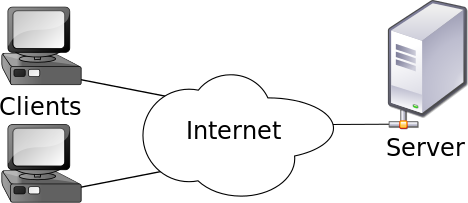
\includegraphics[width=50mm]{images/client-server-model.png}
\caption{Modello client-server}
\end{figure}

La comunicazione è rappresentata da un processo client che manda un messaggio attraverso la rete al processo server e resta in attesa di un messaggio di risposta. Quando il processo server riceve la richiesta esegue il lavoro o recupera i dati desiderati e manda indietro una risposta.

Una rete di calcolatori è un potentissimo \textbf{mezzo di comunicazione}. Alcuni esempi di utilizzo sono i seguenti:

\begin{itemize}

\item Comunicazione tramite \textbf{email};
\item Cooperazione tra gruppi distanti tra loro;
\item Videoconferenze;
\item Realizzare affari in modo elettronico;
\item Commercio elettronico (\textbf{e-commerce});
\item \textbf{Instant messaging};
\item Chat;
\item Comunicazione \textbf{peer-to-peer};
\item Insegnamento a distanza (e-learning);
\item Video on demand;

\end{itemize} 

\subsection{Hardware di rete}

Ci sono due tipi di tecnologie trasmissive impiegate a largo spettro:

\begin{enumerate}

\item Collegamenti broadcast (\textit{broadcast links});
\item Collegamenti punto-punto (\textit{point-to-point links}).

\end{enumerate}

Le \textbf{reti broadcast} hanno un solo canale di comunicazione che è condiviso fra tutte le macchine della rete. Brevi messaggi, chiamati in alcuni contesti \textbf{pacchetti}, sono inviati da ciascuna macchina e ricevuti da tutte le altre. Un campo indirizzo nel pacchetto individua il destinatario, l'indirizzo viene verificato e il pacchetto ricevuto.
\linebreak
\linebreak
Le \textbf{punto-punto}, al contrario, consistono di molte connessioni tra singole coppie di macchine, chiamate \textit{unicasting}. Per andare dalla sorgente alla destinazione, in questo tipo di rete un pacchetto deve visitare una o più macchine intermedie.
\linebreak
\linebreak
Un criterio alternativo per classificare le reti è la loro \textbf{scala}:

\begin{figure}[htbp]
\centering
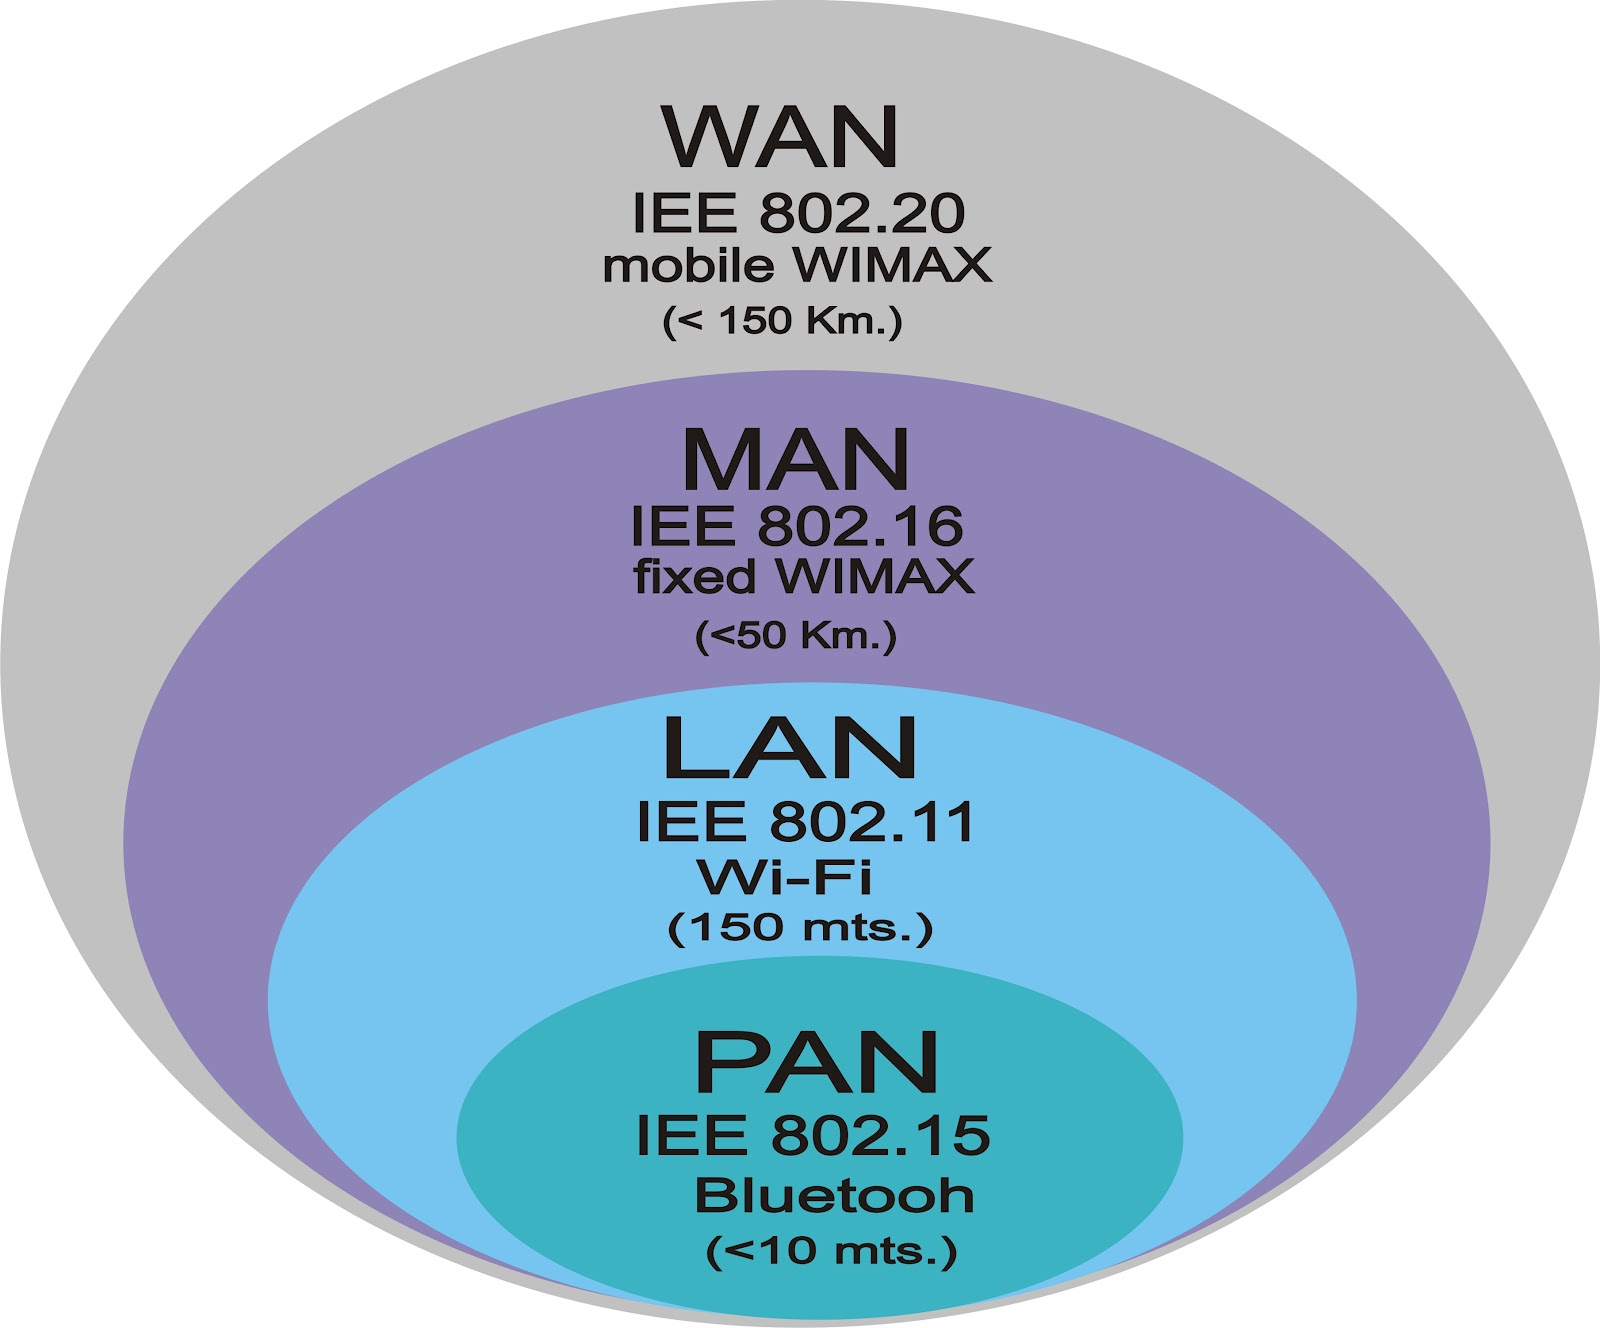
\includegraphics[width=50mm]{images/scala-reti.jpg}
\caption{Classificazione delle reti in base alla scala}
\end{figure}

Le reti locali, solitamente chiamate LAN, sono reti private installate all'interno di un singolo edificio, con dimensione fino a qualche Km, hanno dimensioni contenute e lavorano normalmente a velocità comprese tra 10 Mbps e 100 Mbps. Dispongono di due diverse topologie di trasmissione:

\begin{enumerate}

\item Rete a bus, in cui in ogni istante si può trasmettere a una macchina;
\item Rete ad anello, in cui ogni bit si propaga in modo autonomo senza aspettare il resto del pacchetto;

\end{enumerate}

\begin{figure}[htbp]
\centering
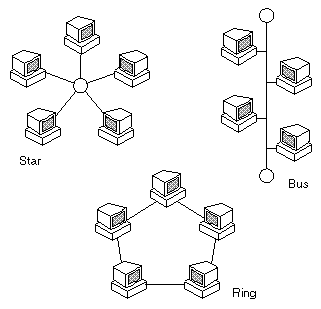
\includegraphics[width=50mm]{images/lan-topologia.png}
\caption{Diverse topologie delle reti LAN}
\end{figure}

Una rete metropolitana (\textit{Metropolitan Area Network}) copre un'intera città. L'esempio più noto di MAN è la rete di televisione via cavo disponibile in molte città degli Stati Uniti. La distribuzione delle informazioni nelle abitazioni avviene tramite una stazione di testa centralizzata.
\linebreak
\linebreak
Una \textit{Wide Area Network} o WAN copre un'area geograficamente estesa, spesso una nazione o un continente. Racchiude una serie di macchine destinate a eseguire programmi utente, chiamate \textbf{host}. Gli host sono collegati da una \textbf{communication subnet}, che trasporta i messaggi da un host all'altro ed è generalmente gestita da una compagnia telefonica o da un Internet provider. Le \textbf{linee di trasmissione} spostano i bit tra le macchine. Gli \textbf{elementi di commutazione} sono computer specializzati che collegano tre o più linee di trasmissione. Quando i dati arrivano da una linea ricevente, l'elemento di commutazione deve scegliere una linea di uscita su cui inoltrarlo. Questo viene eseguito dal \textbf{router}. Il modo in cui un router decide come mandare il messaggio si chiama \textbf{algoritmo di routing}.

\begin{figure}[htbp]
\centering
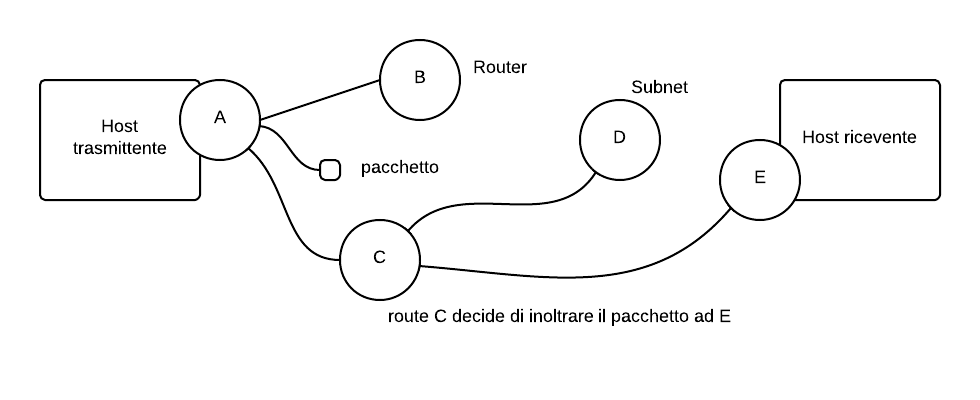
\includegraphics[width=100mm]{images/wan.png}
\caption{Schema di una rete WAN}
\end{figure}

\subsection{Software di rete}

Per diminuire la complessità, la maggior parte delle reti è organizzata come pila di \textbf{strati} (\textit{layer}) o \textbf{livelli}, costruiti uno sull'altro. Lo scopo di ogni strato è quello di offrire determinati servizi agli strati di livello superiore, schermandoli dai dettagli sull'implementazione dei servizi (\textit{information hiding}).
Lo strato \textit{n} di un computer è in comunicazione con lo strato \textit{n} di un altro computer e la comunicazione è regolamentata da \textbf{protocolli}. Fondamentalmente un protocollo è un accordo, tra le parti che comunicano, sul modo in cui deve procedere la comunicazione (formato, ordine in cui i messaggi vengono inviati e ricevuti, azioni da prendere, ...). 
Tra ogni strato contiguo esiste inoltre un'\textbf{interfaccia}, che definisce le operazioni elementari e i servizi che lo strato inferiore rende disponibili a quello soprastante.

\begin{figure}[htbp]
\centering
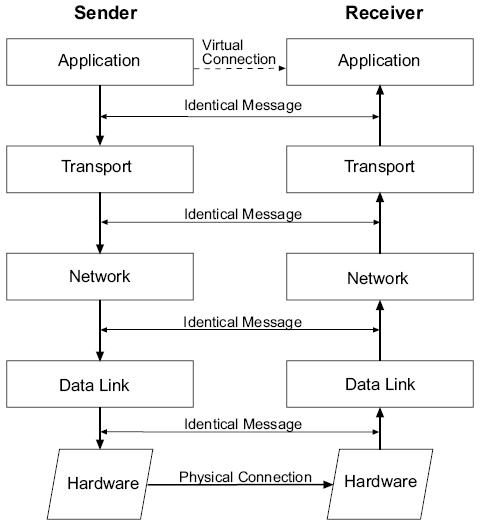
\includegraphics[width=80mm]{images/layers.jpg}
\caption{Organizzazione a strati}
\end{figure}

L'insieme di strati e di protocolli si chiama \textbf{altrorchitettura di rete} (non ne fanno parte le interfacce perchè nascoste dal computer). Un elenco di protocolli usati da uno specifico computer si chiama \textbf{pila di protocolli}.
\linebreak
\linebreak
Gli strati possono offrire due tipi di servizio a quelli sovrastati: orientati alla connessione oppure senza connessione. Un servizio \textbf{orientato alla connessione} assomiglia al sistema telefonico: il trasmettitore spinge gli oggetti (bit) da un estremità (come un tubo) e il ricevitore li prende dall'altra. In alcuni casi il ricevitore e la subnet eseguono una \textbf{negoziazione} dei parametri da usare. 
Al contrario, un servizio \textbf{senza connessione} si comporta come la posta: ogni messaggio trasporta l'indirizzo completo del destinatario ed è instradato attraverso il sistema postale in modo indipendente dagli altri.

\subsection{Il modello di riferimento OSI}

Il modello OSI (\textit{Open System Interconnection}) ha sette strati. I principi che sono stati applicati per arrivare ai sette strati si possono brevemente riassumere come segue:

\begin{enumerate}

\item Si deve creare uno strato quando è richiesta un'astrazione diversa;
\item Ogni strato deve svolgere una funzione ben definita;
\item La funzione di ogni strato va scelta con uno sguardo rivolto alla definizione di protocolli internazionali;
\item I confini degli strati vanno scelti per minimizzare il flusso d'infomrazioni attraverso le interfacce;
\item Il numero di strati deve bastare per evitare la necessità di radunare funzioni distinte nello stesso strato, ma essere abbastanza piccolo da rendere l'architettura instabile.

\end{enumerate}

Lo \textbf{strato fisico} si occupa della trasmissione di bit grezzi sul canale di comunicazione. I requisiti di progetto devono assicurare che ogni bit trasmesso con valore 1 sia ricevuto ancora come 1, e non come 0.
\linebreak
\linebreak
Il compito dello \textbf{strato data link} consiste nel cercare di rilevare, per quanto possibile, gli errori di trasmissione così da evitare di trasmettere questi errori riconosciuti al livello superiore.
\linebreak
\linebreak
Lo \textbf{strato network} controlla il funzionamento della subnet. Un problema chiave riguarda la modalità con cui i pacchetti sono inoltrati dalla sorgente alla destinazione.
\linebreak
\linebreak
La funzione essenziale dello \textbf{strato trasporto} è quella di accettare dati dallo strato superiore, dividerli in unità più piccole quando necessario, passarle allo strato network e assicurarsi che tutti i pezzi arrivino correttamente all'altra estremità.
\linebreak
\linebreak
Lo \textbf{strato applicazione} comprende una varietà di protocolli comunemente richiesti dagli utenti. Un protocollo applicativo largamente utilizzato è HTTP.